
% ----------------------------
% Slide 1: Giới thiệu
% ----------------------------
\begin{frame}[t]
\frametitle{Giới thiệu}
\begin{columns}[T]
    \column{0.5\textwidth}
    Thực hiện thử nghiệm chức năng để xác nhận hệ thống hoạt động đúng thiết kế, bao gồm khởi tạo, kết nối, truyền dữ liệu, phát hiện té ngã và xử lý cảnh báo.
    \begin{itemize}
        \item Log và hình ảnh minh họa các quá trình chính.
    \end{itemize}
    \column{0.5\textwidth}
    % Bên này có thể thêm hình minh họa tổng quan nếu cần
\end{columns}
\end{frame}

% ----------------------------
% Slide 2: Module cảm biến đeo và khởi tạo
% ----------------------------
\begin{frame}[t,fragile]
\frametitle{Module cảm biến đeo và khởi tạo}
\begin{columns}[T]
    \column{0.5\textwidth}
    \begin{itemize}
        \item \textbf{Module 4G/GPS:} Kiểm tra AT command, kết nối 4G, thu nhận GPS. Kết quả: hoạt động ổn định, tọa độ GPS hợp lệ.
        \item \textbf{Khởi tạo hệ thống:} Module SIM4G-GPS, Wi-Fi và tác vụ chính hoạt động bình thường.
    \end{itemize}
    \column{0.5\textwidth}
    \textbf{Log tiêu biểu:}
    \begin{minted}[fontsize=\footnotesize,breaklines]{text}
I (2329) SIM_4G: Received: Quectel EG800K OK
I (34349) SIM_4G: +QGPSLOC: 10.88862,106.77975 OK
I (9961) SIM4G_AT: Initializing SIM4G AT driver...
I (10011) APP_MAIN: System initialization complete.
    \end{minted}
\end{columns}
\vspace{0.2cm}
\textbf{Kết luận:} Hệ thống khởi tạo thành công, tích hợp phần cứng/phần mềm ổn định.
\end{frame}

% ----------------------------
% Slide 3: Kết nối MQTT và truyền dữ liệu
% ----------------------------
\begin{frame}[t,fragile]
\frametitle{Kết nối MQTT và truyền dữ liệu}
\begin{columns}[T]
    \column{0.5\textwidth}
    \begin{itemize}
        \item ESP32 kết nối broker MQTT, gửi bản tin định kỳ (định danh, trạng thái té ngã, GPS).
        \item Dashboard hiển thị dữ liệu MQTT.
    \end{itemize}
    \column{0.5\textwidth}
    \textbf{Log MQTT:}
    \begin{minted}[fontsize=\footnotesize,breaklines]{text}
I (19961) USER_MQTT: MQTT_EVENT_CONNECTED
I (39991) JSON_WRAPPER: Created status payload:
{"device_id":"ESP32_DEV_76E48B","fall_detected":false}
    \end{minted}
    \begin{figure}
        \centering
        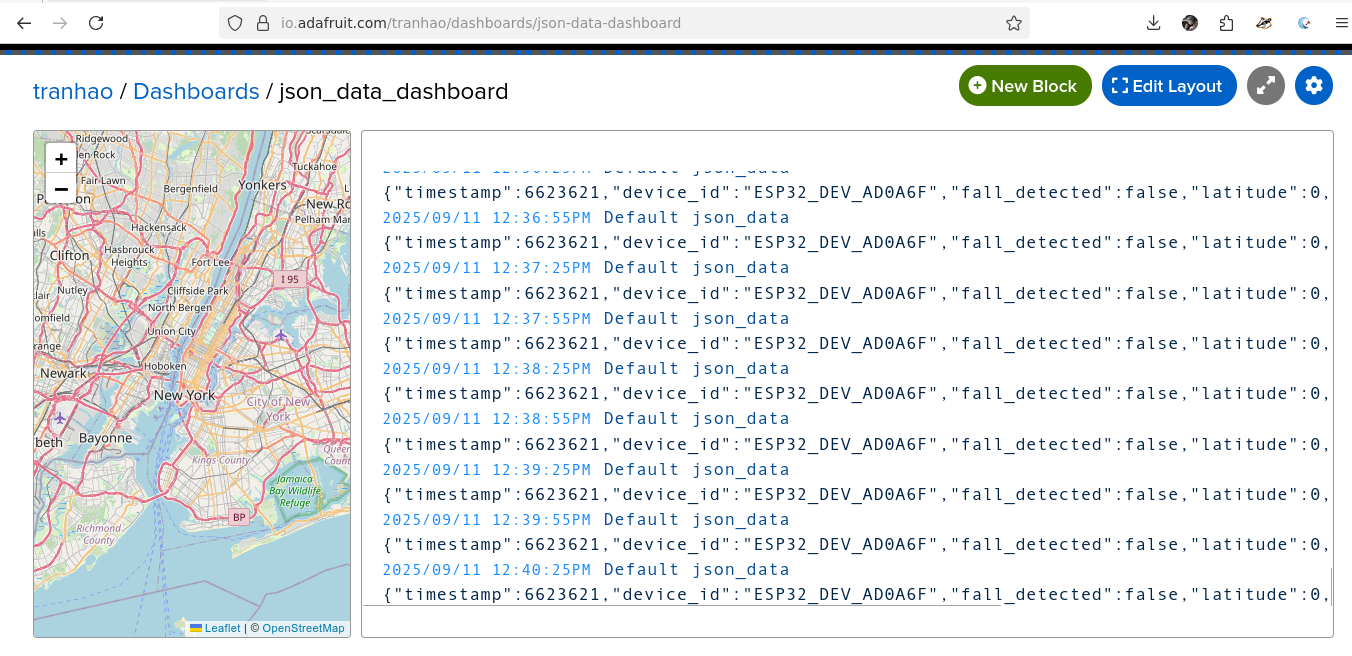
\includegraphics[width=0.9\textwidth]{images/json_data_dashboard.png}
        \caption{Dashboard bản tin MQTT.}
        \label{fig:mqtt_dashboard}
    \end{figure}
\end{columns}
\end{frame}

% ----------------------------
% Slide 4: Phát hiện té ngã và cảnh báo
% ----------------------------
\begin{frame}[t,fragile]
\frametitle{Phát hiện té ngã và cảnh báo}
\begin{columns}[T]
    \column{0.5\textwidth}
    \begin{itemize}
        \item Thuật toán phát hiện té ngã, kích hoạt cảnh báo (SMS, MQTT, buzzer, LED).
        \item Kênh Telegram gửi thông báo từ phần cứng và xử lý hình ảnh.
    \end{itemize}
    \column{0.5\textwidth}
    \textbf{Log phát hiện té ngã:}
    \begin{minted}[fontsize=\footnotesize,breaklines]{text}
E (159131) FALL_LOGIC: FALL DETECTED! Accel: 0.99 g
I (159151) SIM4G_GPS: SMS request queued successfully
I (159191) SIM4G_GPS: MQTT alert published successfully
    \end{minted}
    \begin{figure}
        \centering
        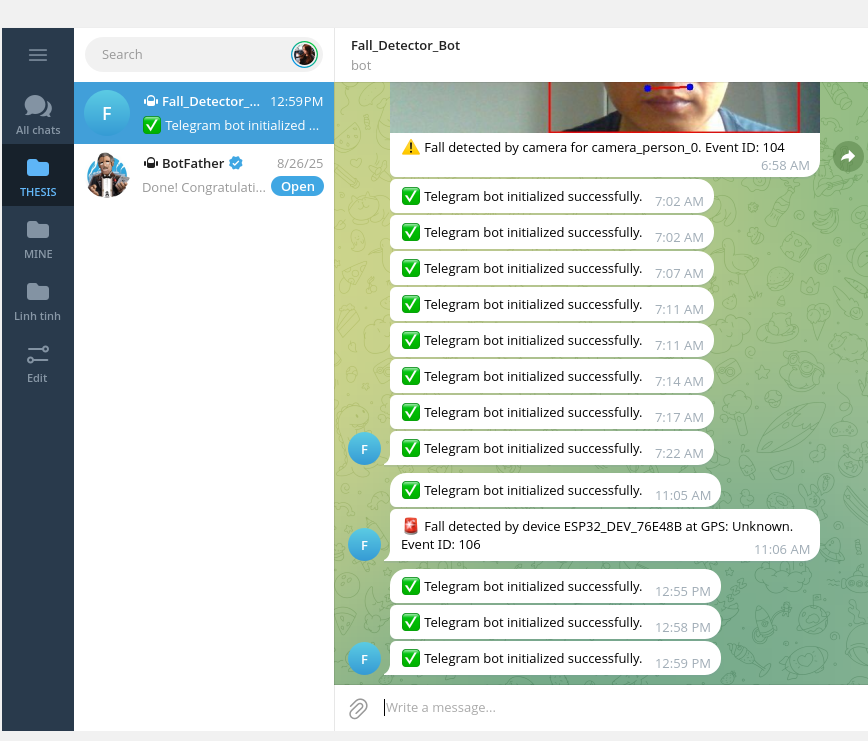
\includegraphics[width=0.9\textwidth]{images/telegram_fall_module1_send.png}
        \caption{Thông báo Telegram từ ESP32.}
        \label{fig:telegram_hw}
    \end{figure}
\end{columns}
\end{frame}

% ----------------------------
% Slide 5: Module Camera và xử lý hình ảnh
% ----------------------------
\begin{frame}[t,fragile]
\frametitle{Module Camera và xử lý hình ảnh}
\begin{columns}[T]
    \column{0.5\textwidth}
    \begin{itemize}
        \item \textbf{Camera:} OV5640 kết nối Wi-Fi, phát luồng HTTP (3.5--5 FPS).
        \item \textbf{Python:} Nhận video, dùng TensorFlow Lite phát hiện người, vẽ skeleton (3--5 FPS).
    \end{itemize}
    \column{0.5\textwidth}
    \textbf{Log camera:}
    \begin{minted}[fontsize=\footnotesize,breaklines]{text}
I (9266) camera: Detected OV5640 camera
I (10006) esp32cam: HTTP server started
I (20006) esp32cam: Frames sent: 50, FPS: 5.87
    \end{minted}
    \begin{figure}
        \centering
        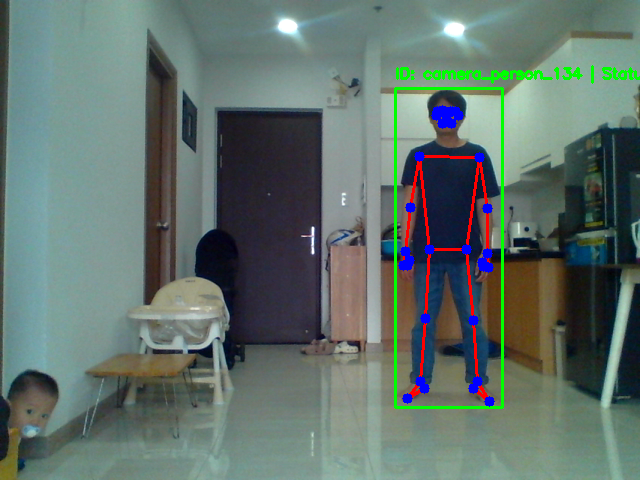
\includegraphics[width=0.9\textwidth]{images/fall_detection_screen_shoot.png}
        \caption{Python phát hiện người và vẽ skeleton.}
        \label{fig:python_skeleton}
    \end{figure}
\end{columns}
\end{frame}

% ----------------------------
% Slide 6: Dữ liệu cảm biến MPU6050
% ----------------------------
\begin{frame}[t]
\frametitle{Dữ liệu cảm biến MPU6050}
\begin{columns}[T]
    \column{0.5\textwidth}
    \begin{table}
        \caption{So sánh đặc trưng}
        \centering
        \footnotesize
        \begin{tabularx}{\textwidth}{|l|X|X|}
            \hline
            \textbf{Thông số} & \textbf{Bình thường} & \textbf{Té ngã} \\
            \hline
            Biên độ Gyro & $\pm 1.5$ dps & $\pm 250$ dps \\
            \hline
            Độ lớn Accel & $\approx 0.95$ g & 0.7--2.0 g \\
            \hline
        \end{tabularx}
    \end{table}
    \column{0.5\textwidth}
    \begin{figure}
        \centering
        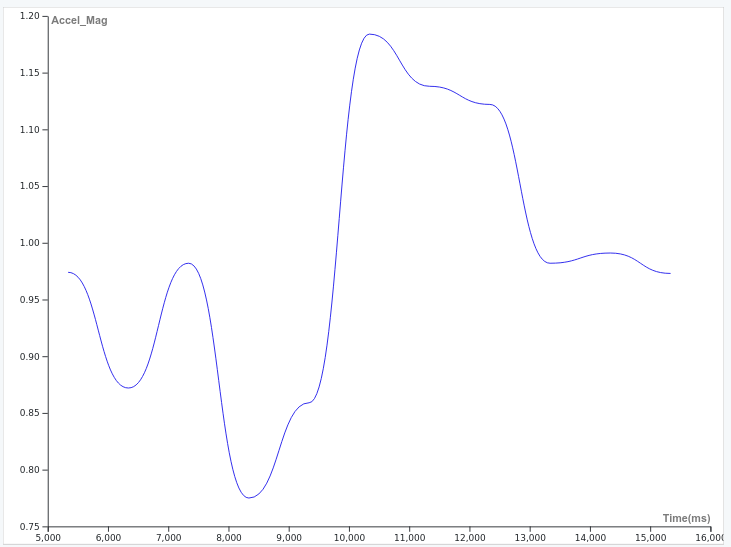
\includegraphics[width=0.9\textwidth]{images/accel_time.png}
        \caption{Biến thiên Accel\_Mag.}
        \label{fig:accel_time}
    \end{figure}
    \begin{itemize}
        \item \textbf{Bình thường:} Accel\_Mag $\approx 1$ g, Gyro\_Mag $\lesssim 2$ dps.
        \item \textbf{Té ngã:} Biến thiên mạnh, Gyro\_Mag lên đến 400 dps.
    \end{itemize}
\end{columns}
\end{frame}

% ----------------------------
% Slide 7: Dữ liệu GPS và Asterisk AMI
% ----------------------------
\begin{frame}[t]
\frametitle{Dữ liệu GPS và Asterisk AMI}
\begin{columns}[T]
    \column{0.5\textwidth}
    \begin{itemize}
        \item \textbf{GPS:} Tọa độ chính xác ($\approx$10.8885, 106.7797), Fix Mode 3, 7 vệ tinh.
        \item \textbf{Asterisk AMI:} Gửi SMS/cuộc gọi đến \texttt{6001}, \texttt{6002} thành công; \texttt{6003} lỗi.
    \end{itemize}
    \column{0.5\textwidth}
    \begin{table}
        \caption{Dữ liệu GPS}
        \centering
        \footnotesize
        \begin{tabular}{|c|c|c|}
            \hline
            \textbf{Time (UTC)} & \textbf{Latitude} & \textbf{Longitude} \\
            \hline
            132517.00 & 10.88854 & 106.77973 \\
            132540.00 & 10.88855 & 106.77973 \\
            \hline
        \end{tabular}
    \end{
